\documentclass[]{article}
\usepackage{lmodern}
\usepackage{amssymb,amsmath}
\usepackage{ifxetex,ifluatex}
\usepackage{fixltx2e} % provides \textsubscript
\ifnum 0\ifxetex 1\fi\ifluatex 1\fi=0 % if pdftex
  \usepackage[T1]{fontenc}
  \usepackage[utf8]{inputenc}
\else % if luatex or xelatex
  \ifxetex
    \usepackage{mathspec}
  \else
    \usepackage{fontspec}
  \fi
  \defaultfontfeatures{Ligatures=TeX,Scale=MatchLowercase}
\fi
% use upquote if available, for straight quotes in verbatim environments
\IfFileExists{upquote.sty}{\usepackage{upquote}}{}
% use microtype if available
\IfFileExists{microtype.sty}{%
\usepackage{microtype}
\UseMicrotypeSet[protrusion]{basicmath} % disable protrusion for tt fonts
}{}
\usepackage[margin=1in]{geometry}
\usepackage{hyperref}
\hypersetup{unicode=true,
            pdftitle={MAthesis},
            pdfborder={0 0 0},
            breaklinks=true}
\urlstyle{same}  % don't use monospace font for urls
\usepackage{natbib}
\bibliographystyle{plainnat}
\usepackage{longtable,booktabs}
\usepackage{graphicx,grffile}
\makeatletter
\def\maxwidth{\ifdim\Gin@nat@width>\linewidth\linewidth\else\Gin@nat@width\fi}
\def\maxheight{\ifdim\Gin@nat@height>\textheight\textheight\else\Gin@nat@height\fi}
\makeatother
% Scale images if necessary, so that they will not overflow the page
% margins by default, and it is still possible to overwrite the defaults
% using explicit options in \includegraphics[width, height, ...]{}
\setkeys{Gin}{width=\maxwidth,height=\maxheight,keepaspectratio}
\IfFileExists{parskip.sty}{%
\usepackage{parskip}
}{% else
\setlength{\parindent}{0pt}
\setlength{\parskip}{6pt plus 2pt minus 1pt}
}
\setlength{\emergencystretch}{3em}  % prevent overfull lines
\providecommand{\tightlist}{%
  \setlength{\itemsep}{0pt}\setlength{\parskip}{0pt}}
\setcounter{secnumdepth}{5}
% Redefines (sub)paragraphs to behave more like sections
\ifx\paragraph\undefined\else
\let\oldparagraph\paragraph
\renewcommand{\paragraph}[1]{\oldparagraph{#1}\mbox{}}
\fi
\ifx\subparagraph\undefined\else
\let\oldsubparagraph\subparagraph
\renewcommand{\subparagraph}[1]{\oldsubparagraph{#1}\mbox{}}
\fi

%%% Use protect on footnotes to avoid problems with footnotes in titles
\let\rmarkdownfootnote\footnote%
\def\footnote{\protect\rmarkdownfootnote}

%%% Change title format to be more compact
\usepackage{titling}

% Create subtitle command for use in maketitle
\newcommand{\subtitle}[1]{
  \posttitle{
    \begin{center}\large#1\end{center}
    }
}

\setlength{\droptitle}{-2em}
  \title{MAthesis}
  \pretitle{\vspace{\droptitle}\centering\huge}
  \posttitle{\par}
  \author{}
  \preauthor{}\postauthor{}
  \date{}
  \predate{}\postdate{}

\usepackage{setspace}
\doublespacing

\begin{document}
\maketitle

\begin{longtable}[]{@{}llrrrr@{}}
\caption{Time bins with age range, epoch name, mean age and
corresponding sample sizes (on individual, species and genus
level)}\tabularnewline
\toprule
bin & EpochBins & MeanBins & nIndividuals & nSpecies &
nGenera\tabularnewline
\midrule
\endfirsthead
\toprule
bin & EpochBins & MeanBins & nIndividuals & nSpecies &
nGenera\tabularnewline
\midrule
\endhead
(0,1e-06{]} & Modern & 0.0000005 & 240 & 58 & 17\tabularnewline
(1e-06,0.0117{]} & Holocene & 0.0058500 & 12 & 6 & 4\tabularnewline
(0.0117,0.126{]} & Upper Pleistocene & 0.0688500 & 46 & 15 &
7\tabularnewline
(0.126,0.781{]} & Middle Pleistocene & 0.4535000 & 46 & 9 &
6\tabularnewline
(0.781,2.59{]} & Lower Pleistocene & 1.6845000 & 68 & 24 &
11\tabularnewline
(2.59,3.6{]} & Upper Pliocene & 3.0940000 & 19 & 12 & 8\tabularnewline
(3.6,5.33{]} & Lower Pliocene & 4.4660000 & 23 & 13 & 8\tabularnewline
(5.33,11.6{]} & Upper Miocene & 8.4700000 & 41 & 21 & 9\tabularnewline
\bottomrule
\end{longtable}

\begin{figure}[htbp]
\centering
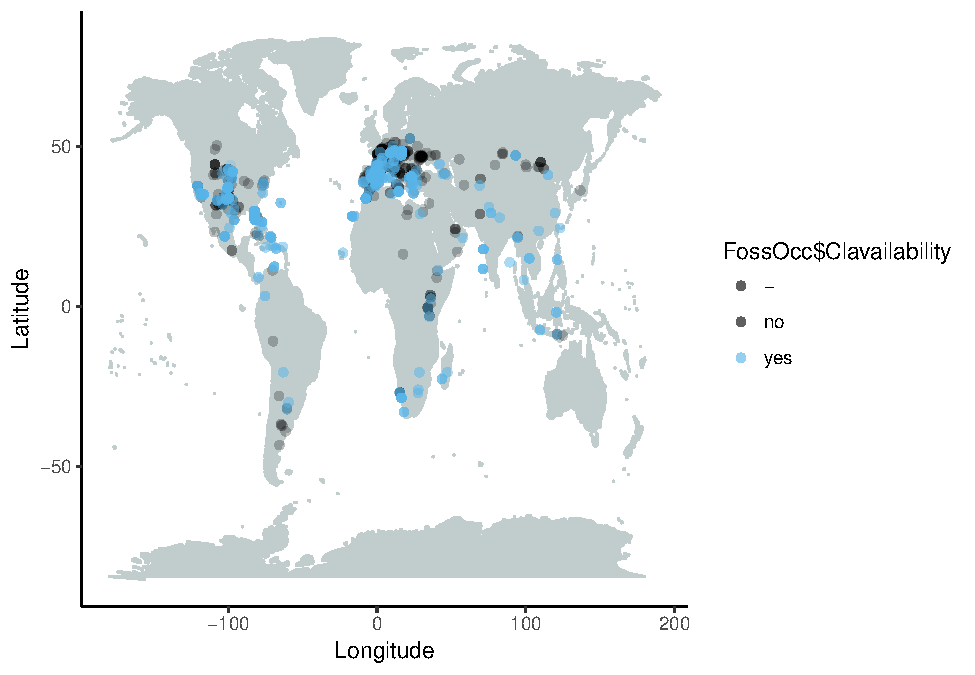
\includegraphics{MA_JJ_files/figure-latex/Map fossil occurrences-1.pdf}
\caption{Map displaying all fossil occurrences of testudinids, with
color indicating whether relevant literature was available (black if
not) and if it was, whether body size data was available or not (yes and
no, respectively).}
\end{figure}

\begin{figure}[htbp]
\centering
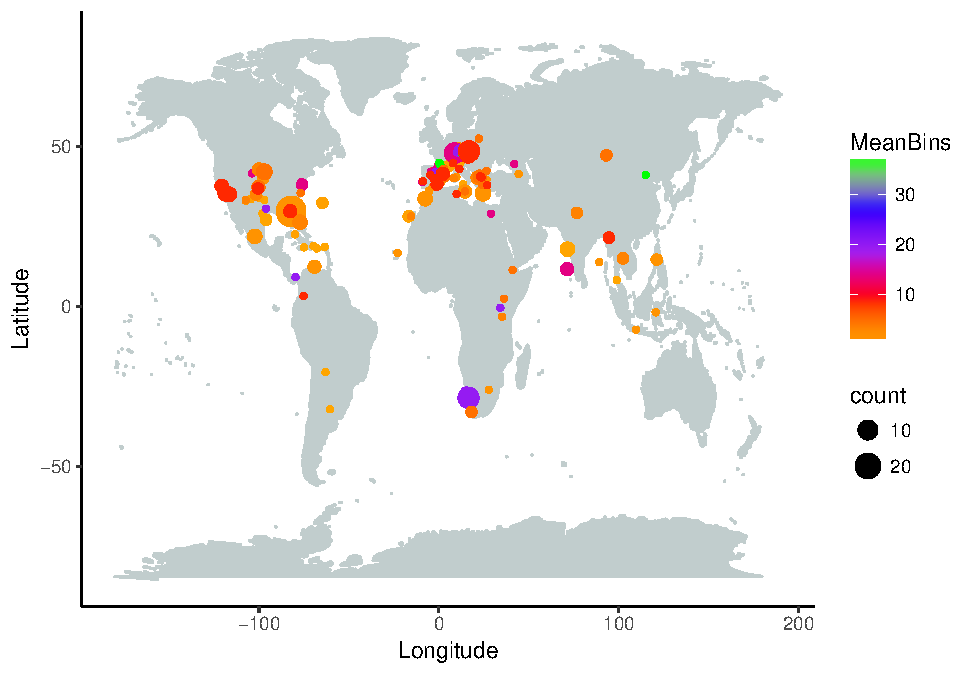
\includegraphics{MA_JJ_files/figure-latex/Map body size data set-1.pdf}
\caption{Map displaying all localities for which body size data for
testudinids was available in the literature. Size of points denotes
sample size, color denotes approximate age.}
\end{figure}

\begin{figure}[htbp]
\centering
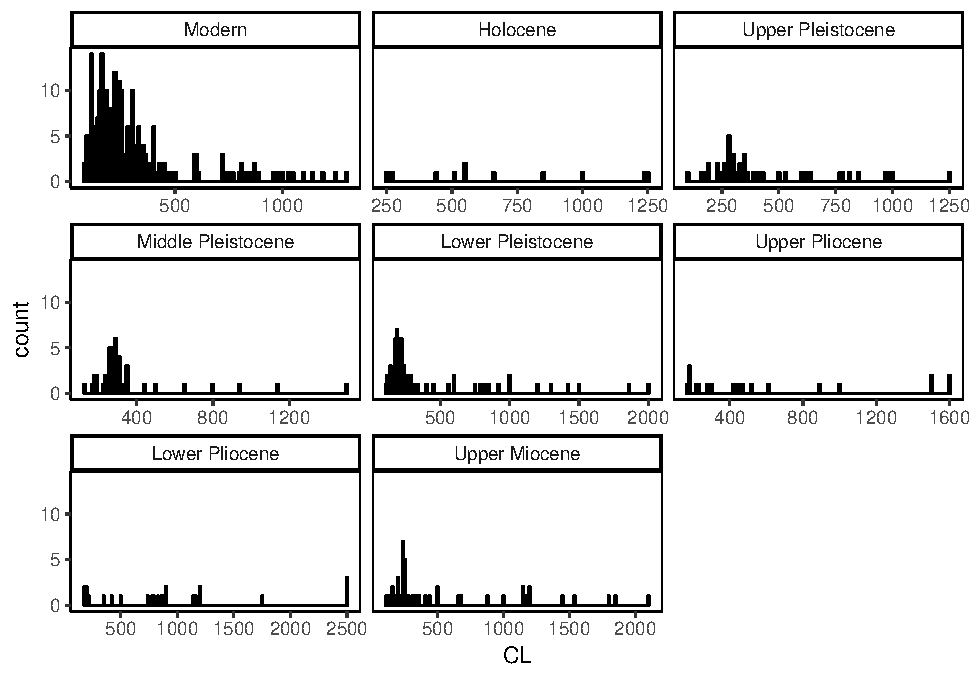
\includegraphics{MA_JJ_files/figure-latex/Histograms of body size data-1.pdf}
\caption{Distribution of body site data per time bin}
\end{figure}

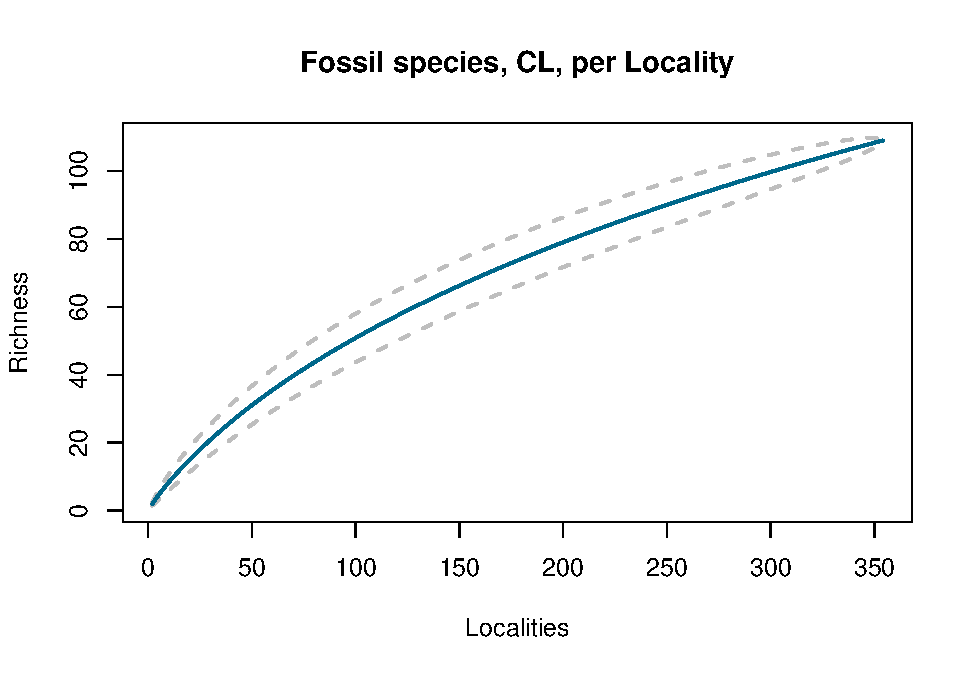
\includegraphics{MA_JJ_files/figure-latex/Species Accumulation Curve-1.pdf}
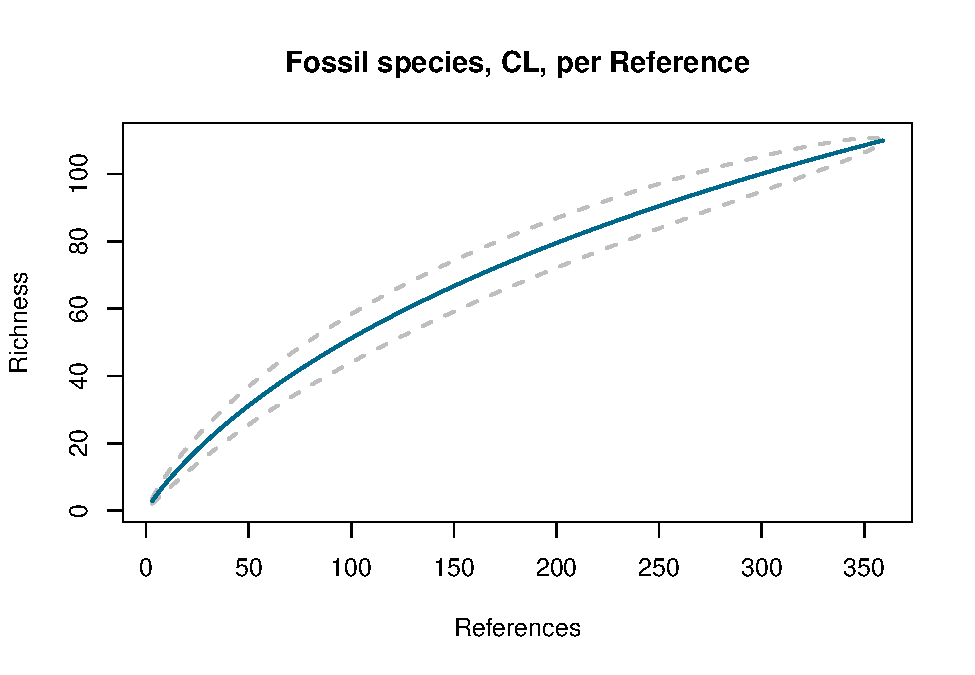
\includegraphics{MA_JJ_files/figure-latex/Species Accumulation Curve-2.pdf}

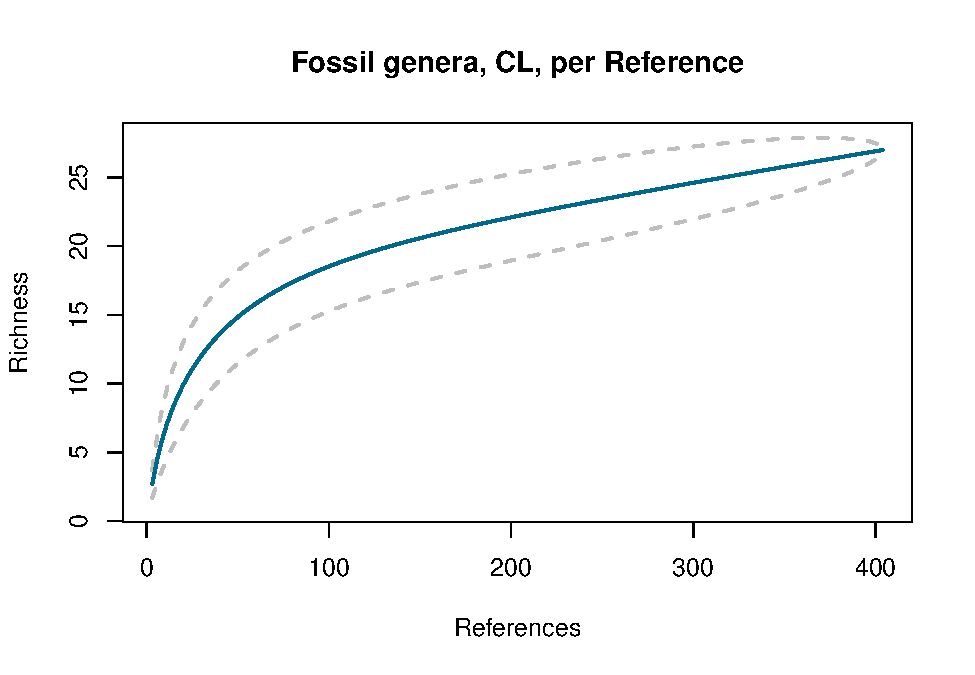
\includegraphics{MA_JJ_files/figure-latex/Species Accumulation Curve with Genera-1.pdf}
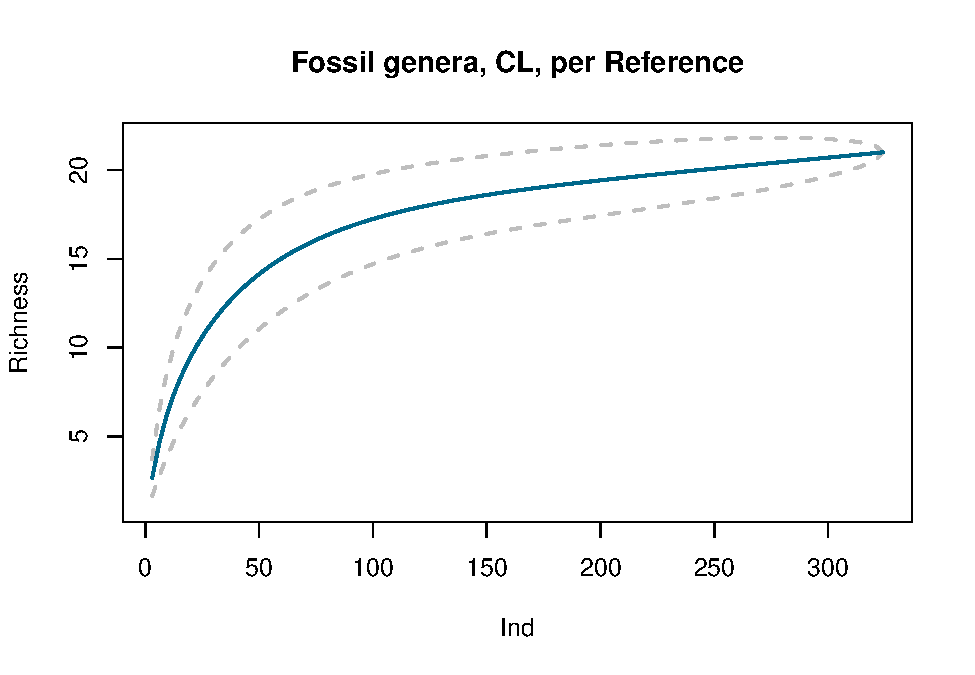
\includegraphics{MA_JJ_files/figure-latex/Species Accumulation Curve with Genera-2.pdf}

\begin{verbatim}
## Warning: Removed 16 rows containing missing values (geom_pointrange).
\end{verbatim}

\begin{figure}[htbp]
\centering
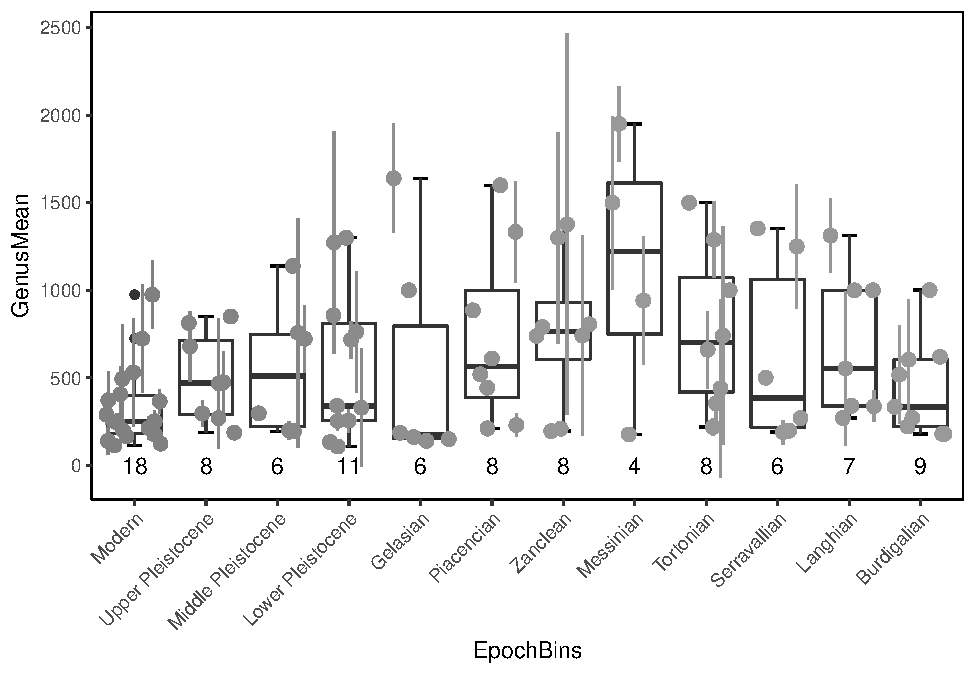
\includegraphics{MA_JJ_files/figure-latex/Boxplots of each genus per time bin-1.pdf}
\caption{Boxplots of each genus per time bin, for colors see Fig. 4.}
\end{figure}

\begin{verbatim}
## Warning: Removed 16 rows containing missing values (geom_pointrange).
\end{verbatim}

\begin{figure}[htbp]
\centering
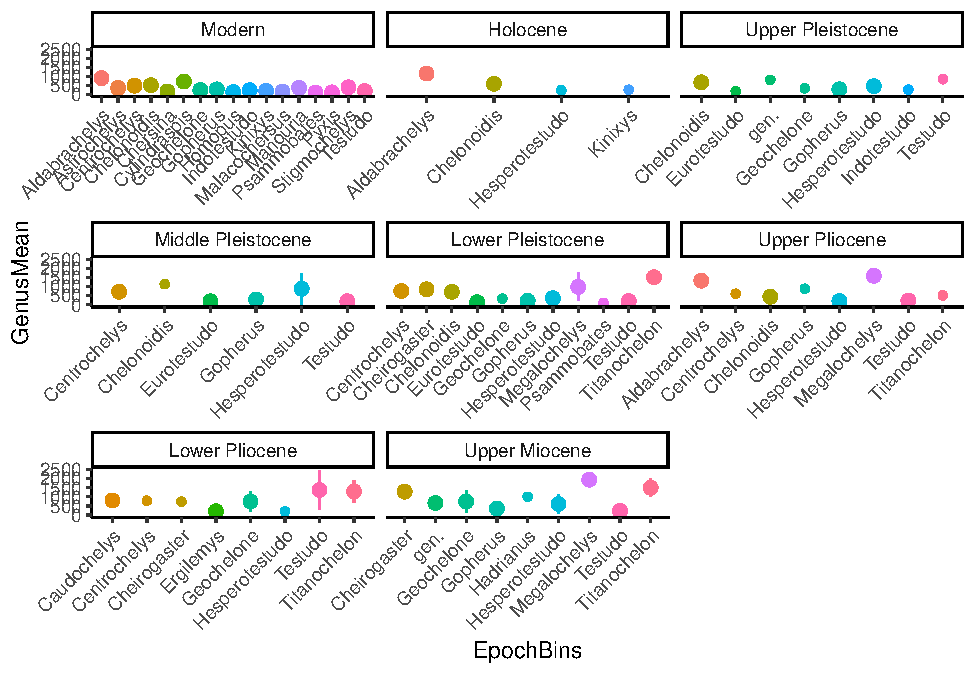
\includegraphics{MA_JJ_files/figure-latex/Separate genera per time bin-1.pdf}
\caption{Mean body size and standard deviation per genus in each time
bin}
\end{figure}

\newpage

\section{including Island species
(n=2215)}\label{including-island-species-n2215}

\begin{longtable}[]{@{}rrrr@{}}
\caption{paleoTS object (mm= mean CL, nn = sample size, vv = variance
(CL), tt = Age)}\tabularnewline
\toprule
mm & nn & vv & tt\tabularnewline
\midrule
\endfirsthead
\toprule
mm & nn & vv & tt\tabularnewline
\midrule
\endhead
246.8335 & 1968 & 2.126636e+09 & 0.0000005\tabularnewline
688.5455 & 11 & 1.245041e+05 & 0.0058500\tabularnewline
447.6480 & 45 & 8.098707e+04 & 0.0688500\tabularnewline
333.8707 & 45 & 3.704545e+04 & 0.4535000\tabularnewline
434.1848 & 66 & 1.967096e+05 & 1.6845000\tabularnewline
642.0167 & 18 & 2.812598e+05 & 3.0940000\tabularnewline
1004.9909 & 22 & 5.319102e+05 & 4.4660000\tabularnewline
582.7750 & 40 & 3.097159e+05 & 8.4700000\tabularnewline
\bottomrule
\end{longtable}

\begin{figure}[htbp]
\centering
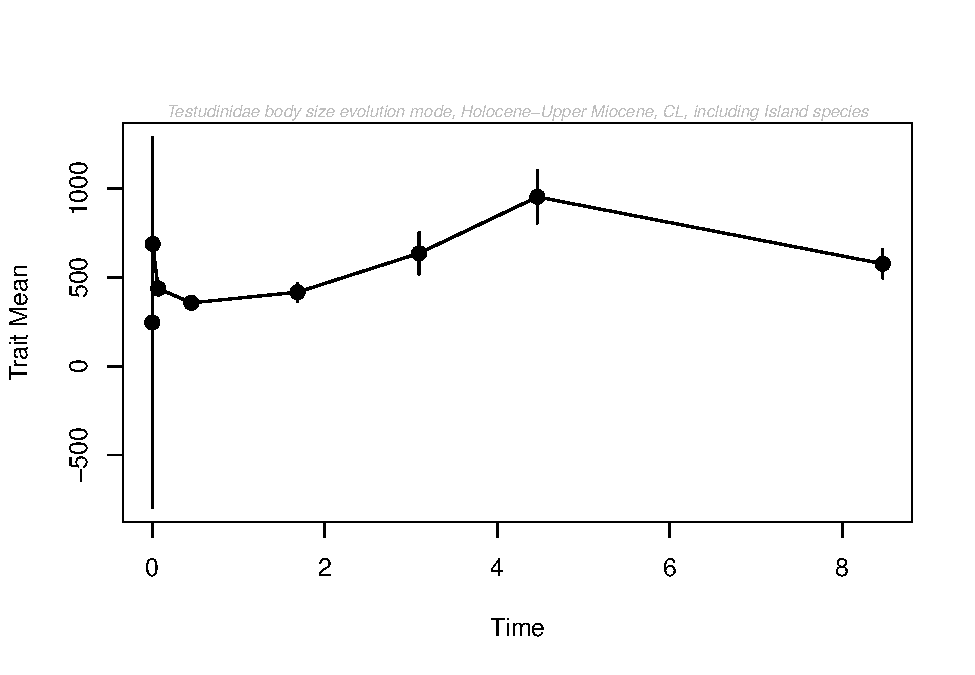
\includegraphics{MA_JJ_files/figure-latex/paleoTS plot-1.pdf}
\caption{individuals, including island species}
\end{figure}

\begin{verbatim}
## 
## Comparing 3 models [n = 7, method = AD]
## 
##             logL K     AICc Akaike.wt
## GRW    -49.84924 2 106.6985     0.044
## URW    -50.76566 1 104.3313     0.145
## Stasis -46.94604 2 100.8921     0.810
\end{verbatim}

\begin{longtable}[]{@{}lrrrr@{}}
\caption{Model-fitting results for testudinidae, individuals, including
island species}\tabularnewline
\toprule
& logL & K & AICc & Akaike.wt\tabularnewline
\midrule
\endfirsthead
\toprule
& logL & K & AICc & Akaike.wt\tabularnewline
\midrule
\endhead
GRW & -49.84924 & 2 & 106.6985 & 0.044\tabularnewline
URW & -50.76566 & 1 & 104.3313 & 0.145\tabularnewline
Stasis & -46.94604 & 2 & 100.8921 & 0.810\tabularnewline
\bottomrule
\end{longtable}

\section{paleoTS plot with species mean, including island
species}\label{paleots-plot-with-species-mean-including-island-species}

\begin{longtable}[]{@{}lrrr@{}}
\toprule
EpochBins & meanSpeciesCL & nSpecies & MeanBins\tabularnewline
\midrule
\endhead
Holocene & 671.4667 & 5 & 0.00585\tabularnewline
Upper Pleistocene & 521.4533 & 17 & 0.06885\tabularnewline
Middle Pleistocene & 384.8626 & 10 & 0.45350\tabularnewline
Lower Pleistocene & 626.2039 & 28 & 1.68450\tabularnewline
Upper Pliocene & 610.4591 & 11 & 3.09400\tabularnewline
Lower Pliocene & 953.9089 & 15 & 4.46600\tabularnewline
Upper Miocene & 680.7708 & 24 & 8.47000\tabularnewline
\bottomrule
\end{longtable}

\begin{longtable}[]{@{}rrrr@{}}
\toprule
tt & mm & vv & nn\tabularnewline
\midrule
\endhead
0.0000005 & 400.5972 & 104321.19 & 50\tabularnewline
0.0058500 & 671.4667 & 195810.92 & 5\tabularnewline
0.0688500 & 521.4533 & 67149.55 & 17\tabularnewline
0.4535000 & 384.8626 & 99603.12 & 10\tabularnewline
1.6845000 & 626.2039 & 335519.43 & 28\tabularnewline
3.0940000 & 610.4591 & 260640.34 & 11\tabularnewline
4.4660000 & 953.9089 & 452469.61 & 15\tabularnewline
8.4700000 & 680.7708 & 349806.99 & 24\tabularnewline
\bottomrule
\end{longtable}

\begin{figure}[htbp]
\centering
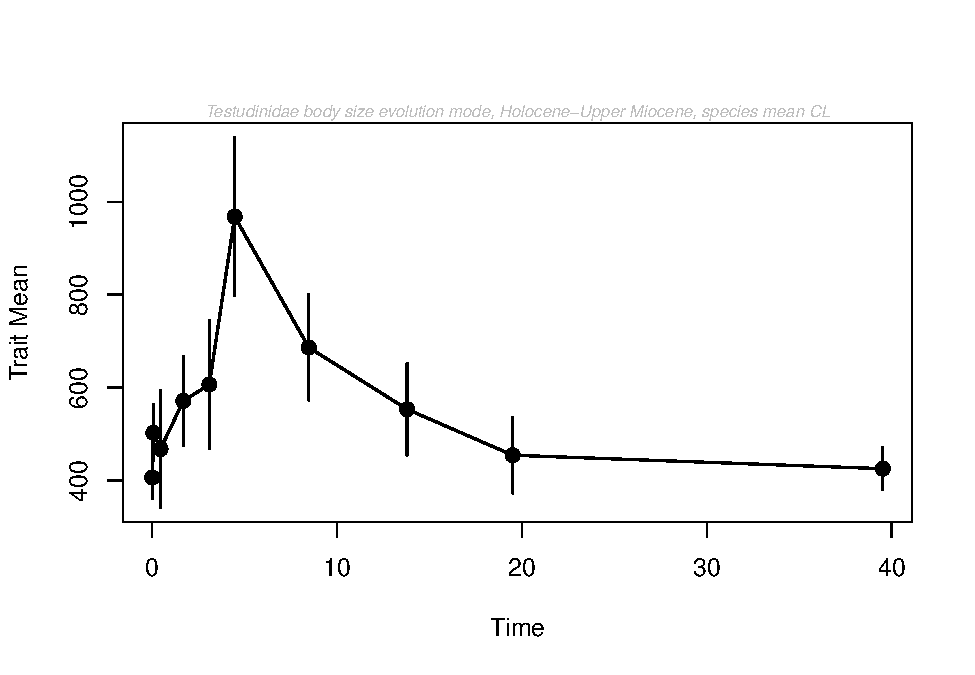
\includegraphics{MA_JJ_files/figure-latex/paleoTS plot with species mean, including island species-1.pdf}
\caption{paleoTS plot with species mean, including island species}
\end{figure}

\begin{verbatim}
## 
## Comparing 3 models [n = 7, method = AD]
## 
##             logL K      AICc Akaike.wt
## GRW    -47.67834 2 102.35667     0.048
## URW    -47.74028 1  98.28056     0.371
## Stasis -45.19334 2  97.38669     0.580
\end{verbatim}

\begin{longtable}[]{@{}lrrrr@{}}
\toprule
& logL & K & AICc & Akaike.wt\tabularnewline
\midrule
\endhead
GRW & -47.67834 & 2 & 102.35667 & 0.048\tabularnewline
URW & -47.74028 & 1 & 98.28056 & 0.371\tabularnewline
Stasis & -45.19334 & 2 & 97.38669 & 0.580\tabularnewline
\bottomrule
\end{longtable}

\newpage

\section{paleoTS plot with genus
mean}\label{paleots-plot-with-genus-mean}

\begin{longtable}[]{@{}rrrrl@{}}
\caption{Overview over body size means per time bin on genus
level.}\tabularnewline
\toprule
CL & n & var & tt & Genus\tabularnewline
\midrule
\endfirsthead
\toprule
CL & n & var & tt & Genus\tabularnewline
\midrule
\endhead
853.3667 & 120 & 168501582 & 5e-07 & Aldabrachelys\tabularnewline
238.6918 & 664 & 372641839 & 5e-07 & Gopherus\tabularnewline
361.0260 & 204 & 412645499 & 5e-07 & Chelonoidis\tabularnewline
140.0327 & 849 & 2949618378 & 5e-07 & Testudo\tabularnewline
366.2143 & 14 & 26286129 & 5e-07 & Astrochelys\tabularnewline
493.3333 & 3 & 2190400 & 5e-07 & Centrochelys\tabularnewline
176.2667 & 15 & 6990736 & 5e-07 & Chersina\tabularnewline
724.0000 & 5 & 13104400 & 5e-07 & Cylindraspis\tabularnewline
252.1250 & 8 & 4068289 & 5e-07 & Geochelone\tabularnewline
139.2857 & 7 & 950625 & 5e-07 & Homopus\tabularnewline
242.9875 & 16 & 15114989 & 5e-07 & Indotestudo\tabularnewline
209.1429 & 14 & 8573184 & 5e-07 & Kinixys\tabularnewline
166.5000 & 2 & 110889 & 5e-07 & Malacochersus\tabularnewline
372.1250 & 8 & 8862529 & 5e-07 & Manouria\tabularnewline
113.4118 & 17 & 3717184 & 5e-07 & Psammobates\tabularnewline
124.1875 & 16 & 3948169 & 5e-07 & Pyxis\tabularnewline
405.3333 & 6 & 5914624 & 5e-07 & Stigmochelys\tabularnewline
\bottomrule
\end{longtable}

\begin{longtable}[]{@{}rrrr@{}}
\toprule
tt & mm & vv & nn\tabularnewline
\midrule
\endhead
0.0000005 & 316.3547 & 44441.20 & 17\tabularnewline
0.0058500 & 568.9167 & 182078.62 & 4\tabularnewline
0.0688500 & 524.0911 & 68449.15 & 7\tabularnewline
0.4535000 & 510.6329 & 170442.90 & 5\tabularnewline
1.6845000 & 615.9960 & 254795.78 & 10\tabularnewline
3.0940000 & 751.0250 & 288801.06 & 8\tabularnewline
4.4660000 & 791.7563 & 187777.18 & 8\tabularnewline
8.4700000 & 883.5611 & 256846.90 & 9\tabularnewline
\bottomrule
\end{longtable}

\begin{figure}[htbp]
\centering
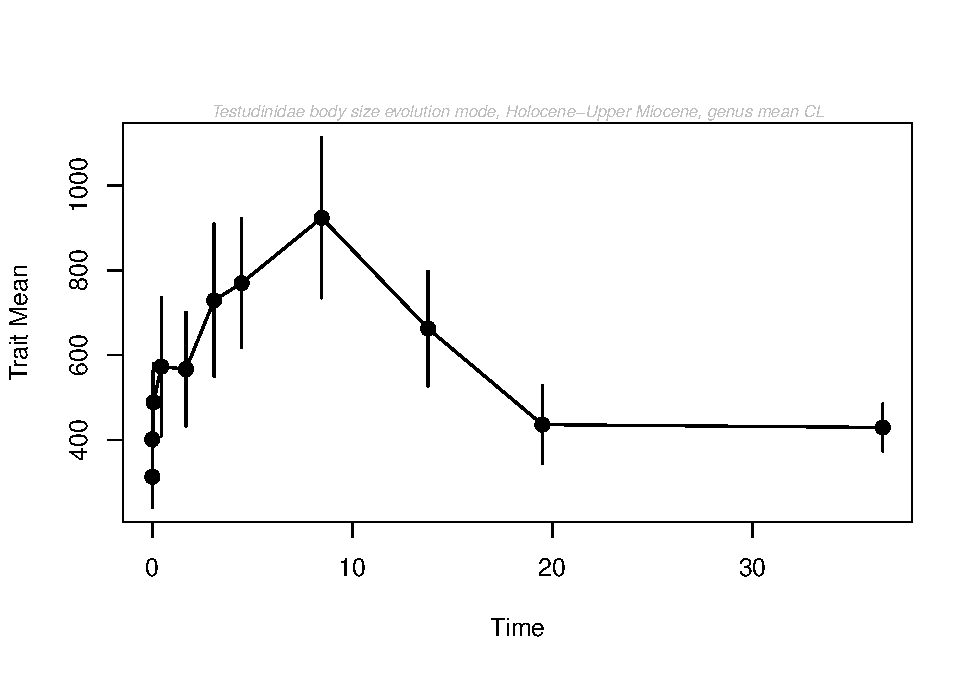
\includegraphics{MA_JJ_files/figure-latex/paleoTS plot with genus mean, including island species-1.pdf}
\caption{paleoTS plot with genus mean, including island species}
\end{figure}

\begin{verbatim}
## 
## Comparing 3 models [n = 7, method = AD]
## 
##             logL K     AICc Akaike.wt
## GRW    -45.37058 2 97.74116     0.107
## URW    -45.58571 1 93.97143     0.702
## Stasis -44.78886 2 96.57771     0.191
\end{verbatim}

\begin{longtable}[]{@{}lrrrr@{}}
\toprule
& logL & K & AICc & Akaike.wt\tabularnewline
\midrule
\endhead
GRW & -45.37058 & 2 & 97.74116 & 0.107\tabularnewline
URW & -45.58571 & 1 & 93.97143 & 0.702\tabularnewline
Stasis & -44.78886 & 2 & 96.57771 & 0.191\tabularnewline
\bottomrule
\end{longtable}

\section{excluding island species}\label{excluding-island-species}

\begin{longtable}[]{@{}rrrr@{}}
\caption{paleoTS object (mm= mean CL, nn = sample size, vv = variance
(CL), tt = Age)}\tabularnewline
\toprule
mm & nn & vv & tt\tabularnewline
\midrule
\endfirsthead
\toprule
mm & nn & vv & tt\tabularnewline
\midrule
\endhead
199.7807 & 1771 & 1.710776e+09 & 0.0000005\tabularnewline
259.0000 & 2 & 1.620000e+02 & 0.0058500\tabularnewline
380.0617 & 35 & 7.471306e+04 & 0.0688500\tabularnewline
274.8795 & 40 & 3.342617e+03 & 0.4535000\tabularnewline
262.7958 & 48 & 6.826984e+04 & 1.6845000\tabularnewline
766.3909 & 11 & 4.261398e+05 & 3.0940000\tabularnewline
1029.0400 & 20 & 5.811355e+05 & 4.4660000\tabularnewline
550.2821 & 39 & 2.745233e+05 & 8.4700000\tabularnewline
\bottomrule
\end{longtable}

\begin{figure}[htbp]
\centering
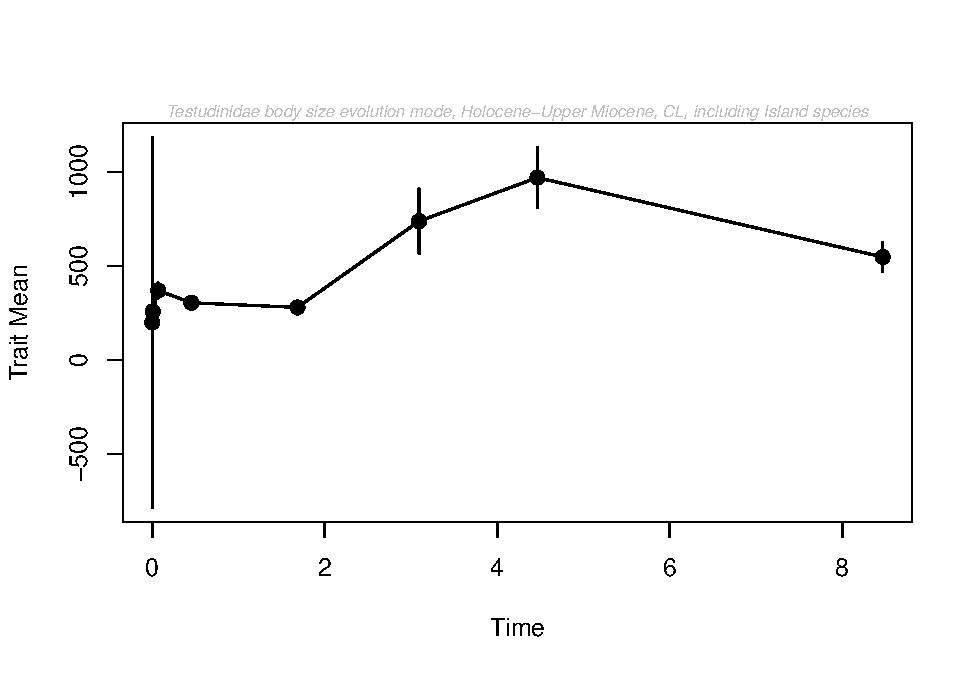
\includegraphics{MA_JJ_files/figure-latex/paleoTS, individuals, exluding island species-1.pdf}
\caption{individuals, excluding island species}
\end{figure}

\begin{verbatim}
## 
## Comparing 3 models [n = 7, method = AD]
## 
##             logL K     AICc Akaike.wt
## GRW    -50.91308 2 108.8262     0.054
## URW    -50.33951 1 103.4790     0.784
## Stasis -49.81453 2 106.6291     0.162
\end{verbatim}

\begin{longtable}[]{@{}lrrrr@{}}
\caption{Model-fitting results for testudinidae, individuals, including
island species}\tabularnewline
\toprule
& logL & K & AICc & Akaike.wt\tabularnewline
\midrule
\endfirsthead
\toprule
& logL & K & AICc & Akaike.wt\tabularnewline
\midrule
\endhead
GRW & -50.91308 & 2 & 108.8262 & 0.054\tabularnewline
URW & -50.33951 & 1 & 103.4790 & 0.784\tabularnewline
Stasis & -49.81453 & 2 & 106.6291 & 0.162\tabularnewline
\newpage & & & &\tabularnewline
\bottomrule
\end{longtable}

\section{paleoTS plot with species mean, excluding island
species}\label{paleots-plot-with-species-mean-excluding-island-species}

\begin{longtable}[]{@{}lrrr@{}}
\toprule
EpochBins & meanSpeciesCL & nSpecies & MeanBins\tabularnewline
\midrule
\endhead
Holocene & 259.0000 & 2 & 0.00585\tabularnewline
Upper Pleistocene & 447.7325 & 12 & 0.06885\tabularnewline
Middle Pleistocene & 248.3908 & 8 & 0.45350\tabularnewline
Lower Pleistocene & 368.7943 & 16 & 1.68450\tabularnewline
Upper Pliocene & 702.4714 & 7 & 3.09400\tabularnewline
Lower Pliocene & 983.0487 & 13 & 4.46600\tabularnewline
Upper Miocene & 629.9348 & 23 & 8.47000\tabularnewline
\bottomrule
\end{longtable}

\begin{longtable}[]{@{}rrrr@{}}
\toprule
tt & mm & vv & nn\tabularnewline
\midrule
\endhead
0.0000005 & 215.4494 & 9193.970 & 32\tabularnewline
0.0058500 & 259.0000 & 162.000 & 2\tabularnewline
0.0688500 & 447.7325 & 71037.951 & 12\tabularnewline
0.4535000 & 248.3908 & 9244.191 & 8\tabularnewline
1.6845000 & 368.7943 & 192142.503 & 16\tabularnewline
3.0940000 & 702.4714 & 393708.572 & 7\tabularnewline
4.4660000 & 983.0487 & 520873.653 & 13\tabularnewline
8.4700000 & 629.9348 & 300864.767 & 23\tabularnewline
\bottomrule
\end{longtable}

\begin{figure}[htbp]
\centering
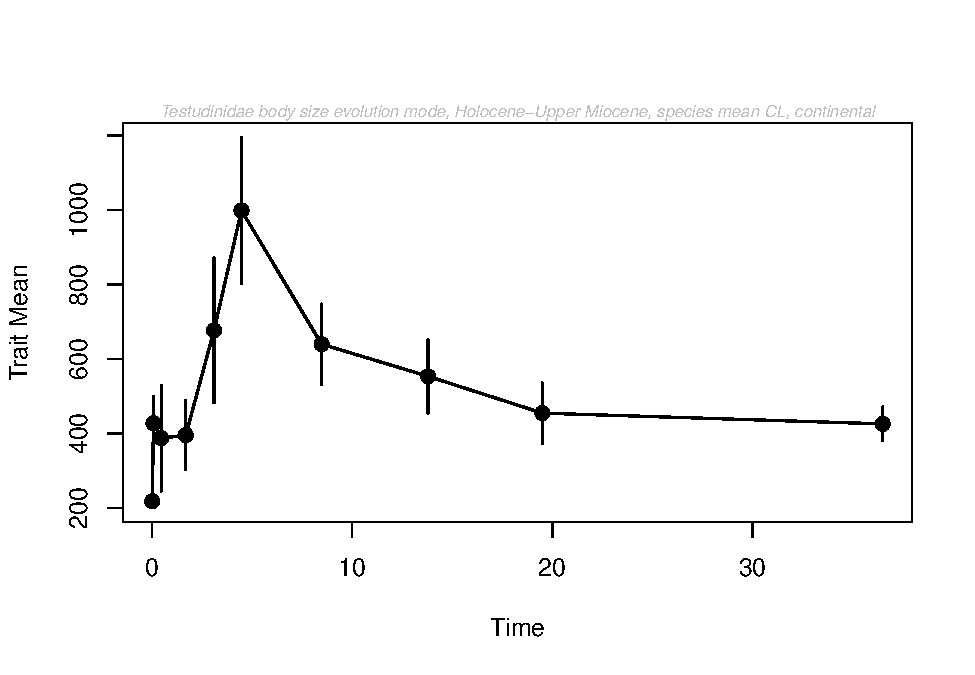
\includegraphics{MA_JJ_files/figure-latex/paleoTS plot with species mean, excluding island species-1.pdf}
\caption{paleoTS plot with species mean, excluding island species}
\end{figure}

\begin{verbatim}
## 
## Comparing 3 models [n = 7, method = AD]
## 
##             logL K     AICc Akaike.wt
## GRW    -48.11009 2 103.2202     0.155
## URW    -48.73586 1 100.2717     0.678
## Stasis -48.03479 2 103.0696     0.167
\end{verbatim}

\begin{longtable}[]{@{}lrrrr@{}}
\toprule
& logL & K & AICc & Akaike.wt\tabularnewline
\midrule
\endhead
GRW & -48.11009 & 2 & 103.2202 & 0.155\tabularnewline
URW & -48.73586 & 1 & 100.2717 & 0.678\tabularnewline
Stasis & -48.03479 & 2 & 103.0696 & 0.167\tabularnewline
\bottomrule
\end{longtable}

\newpage

\section{paleoTS plot with genus
mean}\label{paleots-plot-with-genus-mean-1}

\begin{longtable}[]{@{}rrrrl@{}}
\caption{Overview over body size means per time bin on genus level,
excluding island species.}\tabularnewline
\toprule
CL & n & var & tt & Genus\tabularnewline
\midrule
\endfirsthead
\toprule
CL & n & var & tt & Genus\tabularnewline
\midrule
\endhead
238.4562 & 661 & 373850751 & 5e-07 & Gopherus\tabularnewline
321.4059 & 188 & 368044537 & 5e-07 & Chelonoidis\tabularnewline
139.1260 & 835 & 2997045249 & 5e-07 & Testudo\tabularnewline
493.3333 & 3 & 2190400 & 5e-07 & Centrochelys\tabularnewline
161.6545 & 11 & 3161995 & 5e-07 & Chersina\tabularnewline
256.7143 & 7 & 3229209 & 5e-07 & Geochelone\tabularnewline
139.2857 & 7 & 950625 & 5e-07 & Homopus\tabularnewline
248.1083 & 12 & 8864315 & 5e-07 & Indotestudo\tabularnewline
209.1429 & 14 & 8573184 & 5e-07 & Kinixys\tabularnewline
166.5000 & 2 & 110889 & 5e-07 & Malacochersus\tabularnewline
372.1250 & 8 & 8862529 & 5e-07 & Manouria\tabularnewline
113.2500 & 16 & 3283344 & 5e-07 & Psammobates\tabularnewline
108.0000 & 1 & 11664 & 5e-07 & Pyxis\tabularnewline
405.3333 & 6 & 5914624 & 5e-07 & Stigmochelys\tabularnewline
\bottomrule
\end{longtable}

\begin{longtable}[]{@{}rrrr@{}}
\toprule
tt & mm & vv & nn\tabularnewline
\midrule
\endhead
0.0000005 & 240.8882 & 14018.014 & 14\tabularnewline
0.0058500 & 259.0000 & 162.000 & 2\tabularnewline
0.0688500 & 426.8276 & 57540.323 & 5\tabularnewline
0.4535000 & 230.5548 & 3353.731 & 3\tabularnewline
1.6845000 & 395.5642 & 257838.017 & 6\tabularnewline
3.0940000 & 887.5900 & 439366.116 & 5\tabularnewline
4.4660000 & 800.8417 & 262231.740 & 6\tabularnewline
8.4700000 & 787.1722 & 319006.887 & 9\tabularnewline
\bottomrule
\end{longtable}

\begin{figure}[htbp]
\centering
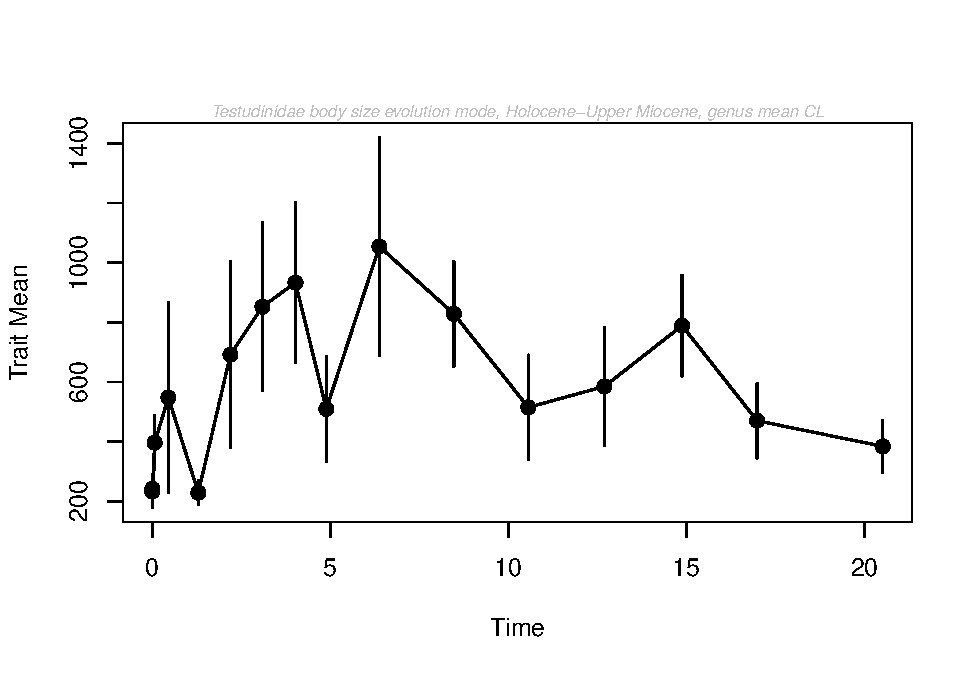
\includegraphics{MA_JJ_files/figure-latex/paleoTS plot with genus mean, excluding island species-1.pdf}
\caption{paleoTS plot with genus mean, excluding island species}
\end{figure}

\begin{verbatim}
## 
## Comparing 3 models [n = 7, method = AD]
## 
##             logL K      AICc Akaike.wt
## GRW    -46.23366 2  99.46732     0.110
## URW    -46.25371 1  95.30742     0.880
## Stasis -48.57439 2 104.14878     0.011
\end{verbatim}

\begin{longtable}[]{@{}lrrrr@{}}
\toprule
& logL & K & AICc & Akaike.wt\tabularnewline
\midrule
\endhead
GRW & -46.23366 & 2 & 99.46732 & 0.110\tabularnewline
URW & -46.25371 & 1 & 95.30742 & 0.880\tabularnewline
Stasis & -48.57439 & 2 & 104.14878 & 0.011\tabularnewline
\bottomrule
\end{longtable}

\newpage

\section{Boxplots (continental (n) vs.~Island (y)
species)}\label{boxplots-continental-n-vs.island-y-species}

\begin{figure}[htbp]
\centering
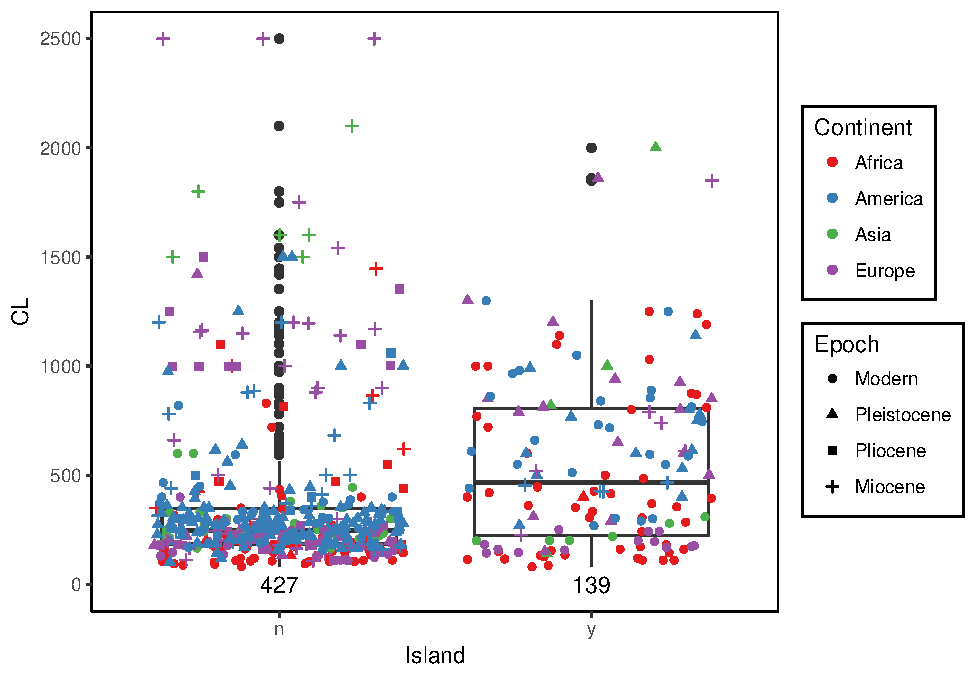
\includegraphics{MA_JJ_files/figure-latex/Boxplot continental vs. insular, individuals-1.pdf}
\caption{Boxplot continental vs.~insular, individuals}
\end{figure}

\begin{figure}[htbp]
\centering
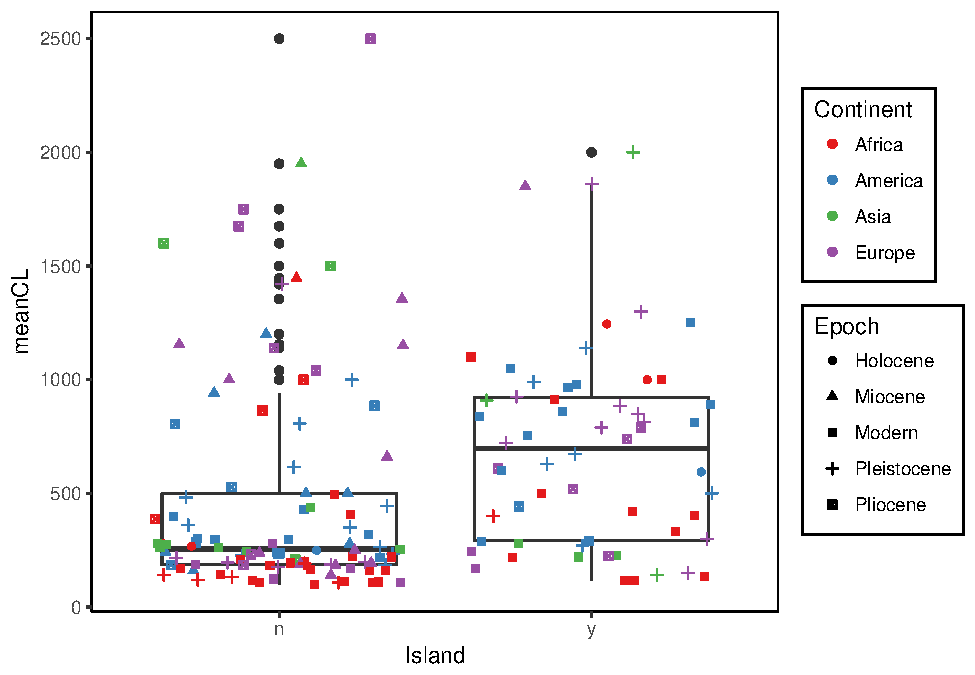
\includegraphics{MA_JJ_files/figure-latex/Boxplots, genera summarised-1.pdf}
\caption{Boxplots continental vs.~insular, genera summarised}
\end{figure}

\begin{figure}[htbp]
\centering
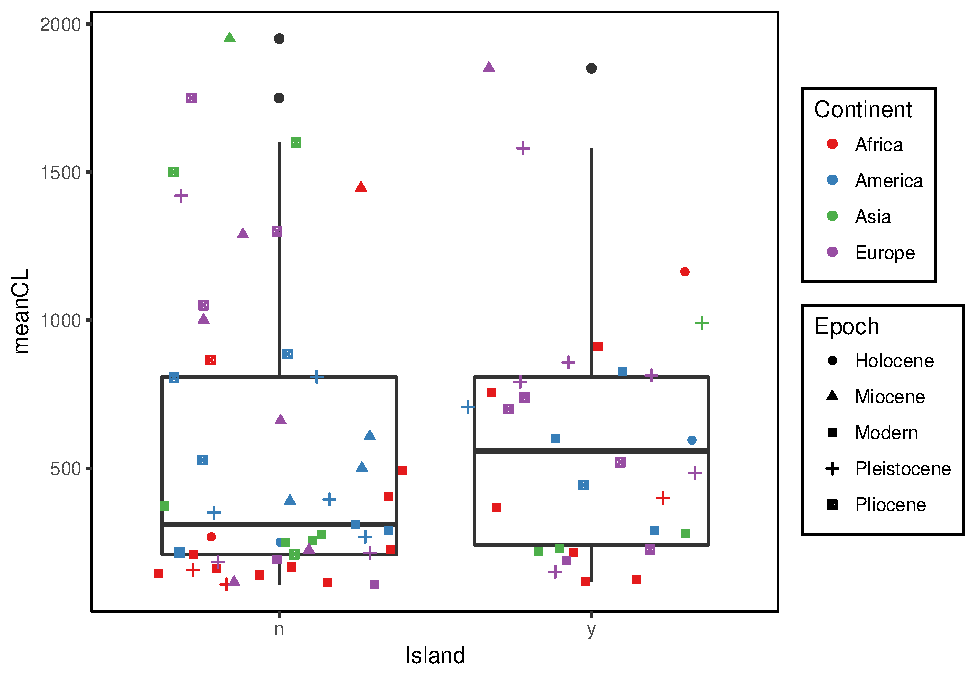
\includegraphics{MA_JJ_files/figure-latex/Boxplot continental vs. insular, species summarised-1.pdf}
\caption{Boxplot continental vs.~insular, species summarised}
\end{figure}

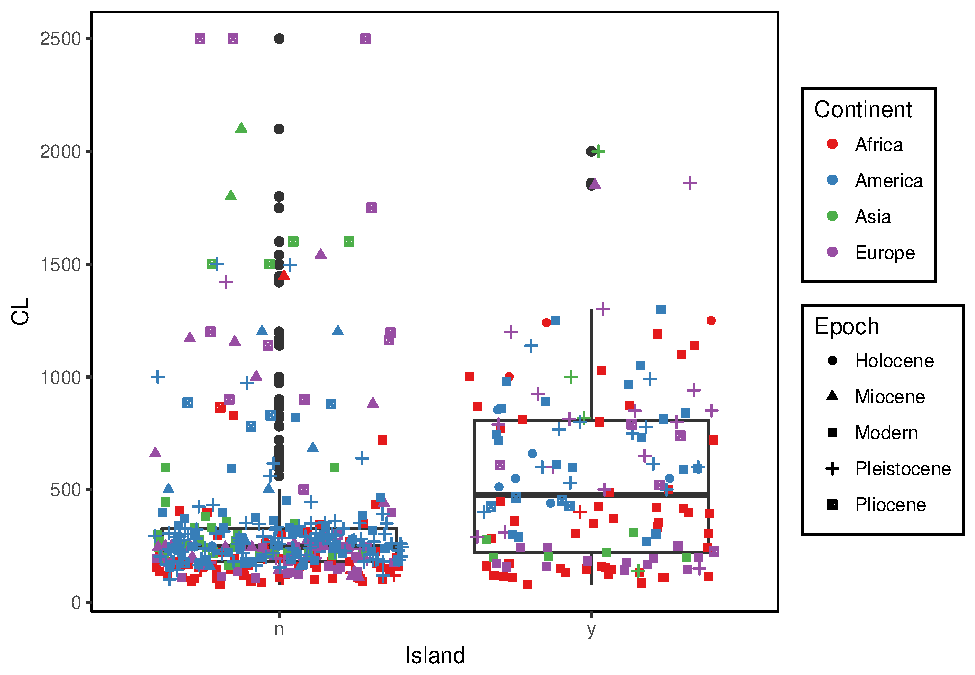
\includegraphics{MA_JJ_files/figure-latex/unnamed-chunk-1-1.pdf}


\end{document}
